%%%%%%%%%%%%%%%%%%%%%%%%%%%%%%%%%%%%%%%%%%%%%%%%%%%%%%%%%%%%%%%%%%%%%%%%%%%%%%%%%%%%%%%%%%%%%%%%%%%%
% ==================================================================================================
% --------------------------------------------------------------------------------------------------
\chapter{Introduction}\label{ch-intro}
Digitization of medical imaging has facilitated
innumerable advances in disease understanding and treatment.
From multi-modal image fusion to image guided therapy, software tools now underpin
research and clinical workflows in almost every domain of medical imaging.
\par
This work concerns an unsolved segmentation problem in 3D brain magnetic resonance imaging (MRI),
in which the objective is to automatically predict the
class, or label, of every voxel (``volume pixel'') in the image.
The objects of interest are white matter hyperintensities (WMH),
non-cancerous brain lesions which are correlated with several neurodegenerative diseases.
This chapter
presents the motivation for automated WMH segmentation,
gives a problem definition,
explores the previously proposed solutions,
and briefly introduces the algorithm proposed in this work.
%%%%%%%%%%%%%%%%%%%%%%%%%%%%%%%%%%%%%%%%%%%%%%%%%%%%%%%%%%%%%%%%%%%%%%%%%%%%%%%%%%%%%%%%%%%%%%%%%%%%
\section{Background}
The brain is composed of three major classes of tissue:
grey matter (GM), white matter (GM), and cerebrospinal fluid (CSF).
Grey matter constitutes the peripheral surface of the brain
-- the cortex, approximately \SI{5}{\milli\metre} thick --
as well as some deeper structures called the basal ganglia.
It contains neuronal cell bodies, and performs the bulk of neural processing.
The white matter is composed primarily of myelinated axons,
and functions to relay information between different GM structures in the brain.
The brain is surrounded by CSF, which provides mechanical and immunological defence.
It is produced by the choroid plexuses in the ventricles of the brain
-- a series of 4 connected cavities.
% ==================================================================================================
\subsection{Magnetic Resonance Imaging}\label{ss:mri}
Magnetic resonance imaging (MRI) provides superior and flexible brain tissue contrast
versus computed tomography (CT) imaging, and is the primary modality for imaging brain disease.
Whereas CT measures tissue density via attenuation of transmitted X-rays,
which does not vary significantly among brain tissues,
MRI measures a mutable combination of 3 tissue characteristics: the proton density (PD),%
\footnote{MRI can be used to image any nucleus with a net nuclear dipole,
  but proton (hydrogen) imaging is most common since hydrogen is biologically abundant
  and gives a strong signal intensity.}
and T1 and T2 relaxation constants~\cite{Pooley2005}.
The physics of signal generation are described below.
\par
\begin{figure}[b]
  \centering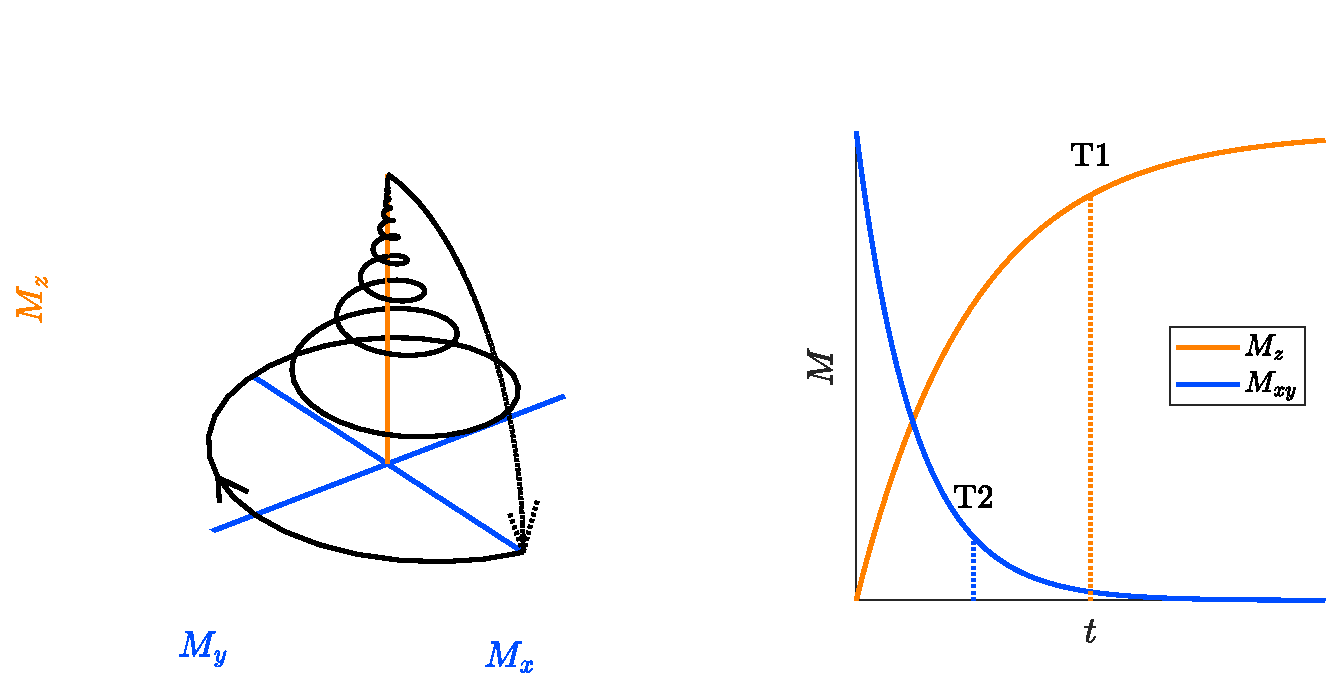
\includegraphics[width=\plotwidth]{mridecay3d}
  \caption{Visualization of T1 and T2 relaxation.}%
  \label{fig:mridecay3d}
\end{figure}
In an MR scanner, a powerful magnetic field induces alignment of proton dipoles with the field.
Only a tiny fraction of the total protons align,
but they create a small magnetic field $M_z$ which is distinct from the main field~\cite{Bloch1946}.
The aligned protons also rotate about the axis of alignment, imperfectly, like a spinning top;
this is called precession, and the frequency of rotation is roughly homogeneous and proportional
to the main field strength~\cite{Bloch1946}.
If a second magnetic field is applied which is \ang{90} perpendicular to the first,
and rotating at the precession frequency, the aligned protons can be forced into
temporary alignment with this transverse rotating field, before decaying
back towards their original state, as illustrated in Figure~\ref{fig:mridecay3d}~\cite{Bloch1946}.
This transient applied magnetic field is induced by a radio frequency (RF) pulse,
and the rate at which the original magnetization $M_z$ is regained is described by
the tissue-specific T1 relaxation constant,
\begin{equation}
  M_z = M_0\et\left(1-e^{-\left(\frac{t}{T1}\right)}\right).%
  \label{eq:T1}
\end{equation}
The T1 constant is dictated by the ability of protons in the tissue to transfer energy
to bonded atoms and surrounding molecules, since this energy transfer defines the transition
from the high energy transverse state to the low energy original state~\cite{Bloch1946,Bryant2005}.
Large macromolecules, membranes, and lipids are generally able to facilitate this energy transfer
more effectively than small molecules like water, producing a shorter T1~\cite{Koenig1990}.
For this reason, myelinated WM has a shorter T1 than GM,
which in turn has a shorter T1 than CSF, which is mostly water~\cite{Roberts2007}.
\par
The rate of decay of the transverse moment $M_{xy}$
is actually not equal to the rate of regeneration of $M_z$.
Rather, this is governed by the T2 relaxation constant,
\begin{equation}
  M_{xy} = M_0\et\left(e^{-\left(\frac{t}{T2}\right)}\right),%
  \label{eq:T2}
\end{equation}
which is always shorter that T1.
This is because, in addition to T1 effects,
the net rotating moment $M_{xy}$ is eroded by proton dephasing.
When precessing protons, having a net dipole, interact with other dipoles or charged particles,
their rotational frequency can be increased or decreased, but overall less coherent,
reducing the perceptible net magnetization $M_{xy}$~\cite{Bloch1946}.
In highly structured tissues like GM and WM, these interactions are more variable,
dephasing is faster, and T2 is shorter~\cite{Roberts2007}.
In fluid environments like CSF, proton interactions are more homogeneous,
yielding longer T2~\cite{Roberts2007}.
For this reason, T2-weighted images are especially useful in identifying pathologies
which degrade tissue structure, since they will have abnormally high T2~\cite{Roberts2007}.
Both relaxation constants depend in a small way on the main magnetic field strength,
measured in Tesla (\si{\tesla}).
T1 and T2 values for various brain tissues at \SI{1.5}{\tesla}
are summarized in Table~\ref{tab:t1t2tissues}.
\par
\begin{table}
  \caption{T1 and T2 constants for brain tissues at 1.5 Tesla.}%
  \label{tab:t1t2tissues}
  \centering{\setlength{\tabcolsep}{2pt}
    \begin{tabular}{ccrclcrclcrclcl}\toprule
      Tissue && \multicolumn{3}{c}{T1 (\si{\milli\second})}
             && \multicolumn{3}{c}{T2 (\si{\milli\second})}
             && \multicolumn{3}{c}{$K [H]$ (a.u.)}
             && Ref\\\midrule
      WM  &&  719 & $\pm$ &  33 &&   73 & $\pm$ &   6 && 0.81 & $\pm$ & 0.03 &&\cite{Schmitt2004}\\
      GM  && 1165 & $\pm$ &  88 &&   92 & $\pm$ &  11 && 0.98 & $\pm$ & 0.07 &&\cite{Schmitt2004}\\
      CSF && 3337 & $\pm$ & 111 && 2562 & $\pm$ & 123 && 1.00 & $\pm$ & 0.07 &&\cite{Schmitt2004}\\
      WML && 1124 & $\pm$ & 372 &&  136 & $\pm$ &  79 &&      &  $-$  &      &&\cite{Stevenson2000}\ss{a}\\
      \bottomrule
  \end{tabular}}
  \tablepost{\ss{a} Estimated from Fig 1 supratentorial data (numerical results not given);
    $\pm$ IQR, not SD; cf.~\S~\ref{ss:WMD} for definition.}
\end{table}
Image acquisition involves sensing the transverse magnetization $M_{xy}$
following proton excitation by an RF pulse.
The problem is that this small signal decays very quickly due to proton dephasing,
which occurs even faster than $T2$ would predict due to a third factor,
inhomogeneity in the main magnetic field~\cite{Chavhan2009}.
The time constant for this decay is termed $T2^*$,
and its effects are usually undesirable~\cite{Chavhan2009}.
As a result, $M_{xy}$ is easily overpowered by the magnetic moment from the RF pulse,
even after it is turned off, due to resonance.
An important solution to this, called the spin-echo,
was proposed by Erwin Hahn in~\citeyear{Hahn1950}~\cite{Hahn1950}.
If $T2^*$ for each proton is assumed to be constant, then reversing the direction of rotation
at a time $t$ should cause all protons to align again at exactly $2t$.
Therefore, at $2t$ the transverse magnetization $M_{xy}$ -- the image signal --
manifests again for sensing, no longer confounded by RF coil resonance~\cite{Hahn1950}.
\par
This second signal is called the Spin Echo ($SE$),
and the interval $2t$ is termed the echo time ($TE$).
Reversing the direction of rotation can be achieved by a \ang{180} RF pulse
at time $TE/2$, in the same way the original excitation is achieved using a \ang{90}
RF pulse (amount of rotation is proportional to the energy of the pulse).
Acquisition of an entire image requires repetitions of this sequence with an interval
called the repetition time ($TR$).
An example spin echo sequence, showing $TE$ and $TR$, as well as $T1$ and $T2$ decay,
is illustrated in Figure~\ref{fig:mrispinecho}.
Spatial encoding for creation of 2D and 3D images
requires the use of additional electromagnetic gradients;
however this topic is omitted here since it is quite complex, and not essential to the current work.%
\footnote{The interested reader is directed to this comprehensive resource on the topic:
  \hreftt{http://mri-q.com/}}
\par
\begin{figure}
  \centering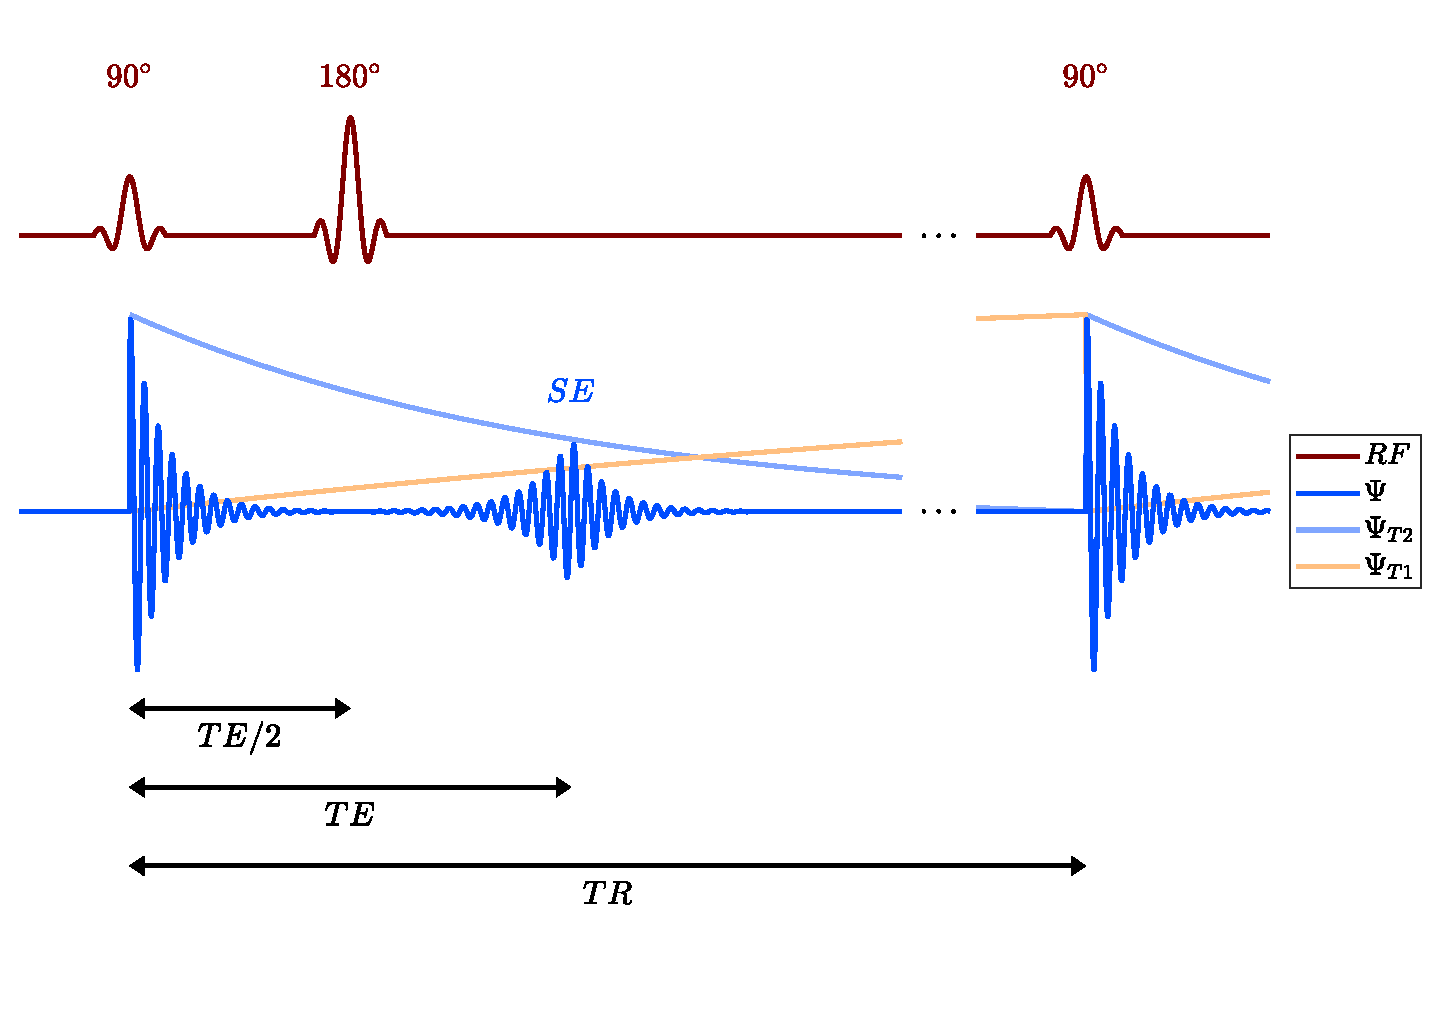
\includegraphics[width=\plotwidth]{mrispinecho}
  \caption{RF and MR signal for a basic Spin Echo sequence.}%
  \label{fig:mrispinecho}
\end{figure}
Using these principals, the nature of MR image contrast can finally be understood.
That is, the signal intensity $\Psi$ for a spin echo sequence at location $x$
can be described by the following 3-term equation,
\begin{equation}\label{eq:MRI-SE}
  \Psi_{SE}(x) = \bigg[K [H](x)\bigg]
    \bigg[e^{-\left(\frac{TE}{T2(x)}\right)}\bigg]
    \bigg[1 - e^{-\left(\frac{TR}{T1(x)}\right)}\bigg],
\end{equation}
where $K$ is scaling factor, and $\left[H\right]$ denotes the proton density.
If $TR$ is chosen to be relatively long,
then the longitudinal magnetization $M_z$ is allowed to recover completely after each repetition,
the third term tends towards 1 for all tissues,
and differences in tissue specific $T1$ are nullified.
Similarly, if $TE$ is relatively short,
then $M_{xy}$ has little time to dephase,
the second term is maintained close to 1,
and differences in $T2$ are nullified.
In order to emphasize differences in $T1$, therefore, $TR$ can be chosen shorter;
for $T2$-weighted contrast, $TE$ can be chosen longer;
and if differences in $[H]$ (proton density, PD) are to be emphasized,
$TR$ can be kept long and $TE$ short.
An example MRI slice using each of these image sequences
is shown in Figure~\ref{fig:4mriT1},~\ref{fig:4mriT2}, and~\ref{fig:4mriPD}.
\par
For identifying WML, T2-weighted images were conventionally used, since the lesions appear bright.
However, CSF in the sulci and ventricles also appears bright on T2 images,
making delineation of lesions -- especially periventricular ones --
difficult in T2 images (Figure~\ref{fig:4mriT2}).
To solve this problem, an adaptation of the spin echo RF pulse sequence can be used,
called an inversion recovery (IR)~\cite{Bydder1985}.
In this sequence, an additional \ang{180} inverting RF pulse is added before the
\ang{90} pulse, so that the longitudinal magnetization $M_z$ is inverted,
then recovers to the original state, passing for a brief moment through zero net magnetization.
The rate of recovery is governed by $T1$, so it is tissue specific.
Furthermore, if the \ang{90} pulse is applied at the instant of zero net magnetization,
no transverse moment will develop, nor the subsequent spin echo.
Therefore this time interval, called the inversion time ($TI$),
can be chosen to null the signal from any tissue with a unique $T1$.
The equation governing the image signal simply adds an inversion term,
\begin{equation}\label{eq:MRI-IR}
  \Psi_{IR}(x) = \bigg[K \left[H(x)\right]\bigg]
    \bigg[e^{-\left(\frac{TE}{T2(x)}\right)}\bigg]
    \bigg[1 + e^{-\left(\frac{TR}{T1(x)}\right)} - 2e^{-\left(\frac{TI}{T1(x)}\right)}\bigg].
\end{equation}
This inversion principal is now often used to null the signal from CSF,
especially for delineation of WMH, in a sequence called
FLuid Attenuation Inversion Recovery (FLAIR)~\cite{Hajnal1992}.
FLAIR images are usually T2-weighted.
Figure~\ref{fig:4mriIR} shows an example FLAIR image, where a WMH can be seen,
posterior to the occipital horn of the left lateral ventricle,
much more clearly than in the T2 image.
\begin{figure}
  \centering
  \begin{subfigure}{0.24\textwidth}
    \includegraphics[width=\textwidth]{i15_training01_01_mprage.png}
    \caption{T1}%
    \label{fig:4mriT1}
  \end{subfigure}
  \begin{subfigure}{0.24\textwidth}
    \includegraphics[width=\textwidth]{i15_training01_01_t2.png}
    \caption{T2}%
    \label{fig:4mriT2}
  \end{subfigure}
  \begin{subfigure}{0.24\textwidth}
    \includegraphics[width=\textwidth]{i15_training01_01_pd.png}
    \caption{PD}%
    \label{fig:4mriPD}
  \end{subfigure}
  \begin{subfigure}{0.24\textwidth}
    \includegraphics[width=\textwidth]{i15_training01_01_flair.png}
    \caption{FLAIR}%
    \label{fig:4mriIR}
  \end{subfigure}
  \caption{Example MRI image set with WMH pathology; from~\cite{WMHSEG2017}.}%
  \label{fig:4mri}
\end{figure}
% ==================================================================================================
\subsection{White Matter Disease}\label{ss:WMD}
``Normal'' ageing of the brain is characterized by a variety of physical and cognitive changes.
Memory, synaptic plasticity, and brain volume decline,
with observable effects on cognitive function~\cite{Peters2006,Good2002}.
Brain ageing is also expedited in many patients by neurodegenerative diseases
targeting the white matter, including
Alzheimer's disease (AD), cerebrovascular disease, and in rare cases Multiple Sclerosis (MS).
While the etiologies of these diseases are not yet fully understood,
there is considerable evidence to suggest that the they are intertwined%
~\cite{Debette2010,Conklin2014,Heppner2015,Snyder2015}.
\par
Cerebrovascular disease describes changes to blood vessels in the brain which increase the risk of
ischemic injury -- a reduction in blood flow due to vessel occlusion or hemorrhage.
Ischemic injuries include
major events (stroke)~\cite{VanderWorp2007},
transient ischemic attacks~\cite{Albers2002}, and
chronic hypoperfusion due to small vessel disease~\cite{Pantoni2010}.
In all such events, neuronal death occurs from insufficient nutrient supply~\cite{VanderWorp2007}.
Strokes involving major cerebral arteries can be fatal,
and post-event quality of life in survivors is highly variable~\cite{Prabhakaran2015}.
In the less dramatic courses, clinically quiet disease progression can lead to
personality changes, memory loss, and reduced cognitive ability;
such changes are termed vascular dementia~\cite{Roman1993}.
\par
Alzheimer's Disease is another subclass of dementia with similar symptoms;
in fact it is the most common type,
affecting about 6\% of the population over age 65~\cite{Burns2009}.
The cause of Alzheimer's disease is hotly debated.
Two 30-year-old theories linking the disease to
the build up of amyloid $\beta$ protein and misfolded protein $\tau$
have been widely supported by correlational studies~\cite{Masters1985,Hardy2002,Lee2011},
but have lacked clear mechanisms of injury until recently.
It is now thought that amyloid $\beta$ oligomers interfere with
neuronal mitochondria and synapse function, leading to cell death~\cite{Kim2013,Tu2014},
while aberrant $\tau$ proteins disrupt microtubules
necessary for intraneuronal transport~\cite{Lee2011}.
During the search for these mechanisms, competing theories implicating
vascular injury~\cite{Snyder2015},
immune response~\cite{Heppner2015},
and blood brain barrier disruption~\cite{Bell2009} have emerged,
painting the picture of a more complex disease.
\par
The pathophysiology of multiple sclerosis is similarly unclear,
though genetics are a necessary factor, and it is known that symptoms arise from erosion of myelin
-- a fatty insulating layer surrounding axons
which is critical for normal neuron firing~\cite{Trapp2008}.
Several theories hypothesize either that this damage is driven by
autoimmune attack, followed by neuronal dysfunction and death,
or that neurodegenerative changes stimulate recruitment of immune cells
as part of the usual response to injury~\cite{Trapp2008,Lucchinetti2000}.
Recent evidence favours the former mechanism,
particularly with inflammatory injury as the initiating event~\cite{Ciccarelli2014,Mahad2015}.
%A helpful visualization of MS lesion progression over one year is available here%
%\footnote{\hreftt{http://www.msdiscovery.org/sites/default/files/MGrid\_crop4\_full\_0.gif}}.
\par
Connecting all these diseases are white matter lesions (WML, \textsc{aka} Leukoariosis),
which represent the macroscopic changes to brain tissue
in regions of white matter damage~\cite{Debette2010,Bakshi2005,Wardlaw2015}.
WML are very common in elderly populations,
and a small volume of lesion does not necessarily implicate one of the above diseases;
in one study of 1077 subjects aged 60-90, 95\% had at least one WML~\cite{DeLeeuw2001}.
WML appear as bright tissue regions in T2-weighted MRI due to some combination of
inflammatory injury and degradation of tissue structure~\cite{Bakshi2005,Wardlaw2015};
in this imaging context, WML are often called white matter hyperintensities (WMH).
Lesions are often focal, as opposed to diffuse, but there is evidence to suggest that
surrounding regions of moderate hyperintensity,
sometimes called ``dirty appearing white matter (DAWM)'',
are also related to the diseases~\cite{Ge2003}.
As biomarkers of the most common WM diseases
-- conditions with unsolved etiologies and inadequate treatments --
WML are of special interest to many brain researchers.
The next section discusses how they are used.
% ==================================================================================================
\subsection{MRI in White Matter Disease}
MR imaging plays important roles in diagnosis and research of white matter diseases.
Typical MRI protocols include T1, T2, and FLAIR sequences,
though only the latter two sequences depict WML as hyperintense~\cite{Simon2006,Wardlaw2013}.
Depending on the disease and context, WMH can be quantified in several ways,
including binary criteria (e.g.\ is there a lesion in a specific location)~\cite{Polman2011},
rating scales (e.g.\ a summary of several criteria)~\cite{Fazekas1987},
or explicit manual segmentation of the lesions by an expert~\cite{Egger2017}.
\par
WMH are arguably most important in MS.
Particularly since WMH are more specific to this disease in younger patients,
WMH have long been used in the diagnosis of MS,
and can even be used to replace some clinical criteria,
as in the 2010 McDonald Criteria~\cite{Polman2011}.
MRI can also be used to discriminate between MS subtypes,
which stratify disease aggression and course~\cite{Polman2011,Lublin2014,Traboulsee2015}.
In numerous clinical trials, WMH have also been used as biomarkers of treatment efficacy%
~\cite{Sormani2013,Fahrbach2013,Ziemssen2015},
since WMH have been shown to be more sensitive to disease progression than clinical features
in certain subtypes~\cite{ORiordan1998}.
In fact, despite the central role of MRI in management and research of MS,
there exists a so-called ``clinico-radiological'' paradox,
which is the surprisingly limited correlation between WMH and clinical MS symptoms
like physical and cognitive impairment~\cite{Mollison2017}.
However, this only strengthens the case for continued WMH research,
particularly considering the recommendations by~\citeauthor{Mollison2017} in~\cite{Mollison2017}
to standardize image analysis in order to better understand the paradox.
\par
In dementia (including vascular and AD),
WMH are used to discriminate between disease subtypes during diagnosis.
For example, the presence of at least one WML was deemed \textit{necessary}
for diagnosis of vascular dementia in~\citeyear{Roman1993}~\cite{Roman1993},
and subsequent revisions to these widely used criteria (NINCDS-ADRDA)
have added this feature as an \textit{exclusionary} criteria for AD~\cite{Dubois2007}.
While diagnosis of additional dementia subtypes may be improved using imaging%
~\cite{Sorbi2012,Verhagen2016}, diagnosis of the most prevalent -- AD --
continues to be based on clinical features alone~\cite{McKhann2011}.
As a result, WMH have not been used as an endpoint to any AD clinical trial.
In fact, only recently have specific standards for
use of WMH in vascular dementia studies been outlined~\cite{Wardlaw2015,Wardlaw2013},
with some subsequent uptake~\cite{VanWesten2016}.
And yet, a~\citeyear{Debette2010} meta-analysis found that
WMH in brain MRI were independently correlated with
stroke risk, dementia (including AD) and death~\cite{Debette2010},
suggesting that much more can be done to make use of WMH as hallmarks of neurodegenerative disease.
%%%%%%%%%%%%%%%%%%%%%%%%%%%%%%%%%%%%%%%%%%%%%%%%%%%%%%%%%%%%%%%%%%%%%%%%%%%%%%%%%%%%%%%%%%%%%%%%%%%%
\section{Problem Statement}
White matter hyperintensities,
as ubiquitous biomarkers of several diseases with unsolved pathophysiology,
are of great interest to brain researchers.
Segmentation of WMH, compared to visual rating scales, provides a finer resolution
for quantification of lesion load, and gives the explicit spatial distribution of pathology.
This spatial information can be very useful,
since diagnostic criteria often consider lesion location~\cite{Sorbi2012}
and there are several correlations between lesion location
and suspected etiology of WMH~\cite{Wardlaw2015,Kim2008}.
\par
Unfortunately, manual segmentation of WMH is
laborious, and subject to large inter- and intra-rater variability, as reported in several works.
Table~\ref{tab:interrater-cite} summarizes these reports,
where similarity index (SI $\in [0,1]$) is a measure of voxel-wise agreement,
and interclass correlation coefficient (ICC $\in [0,1]$) measures total volume agreement
(cf.~\S~\ref{ss:exp-metrics} for definitions).
Table~\ref{tab:interrater-cite} also gives the results using four semi-automated approaches,
since these methods are reported to reduce variability and task time
over strictly manual segmentation.
Yet, for very large scale research studies,
any approach requiring human intervention would be prohibitively time consuming and subjective.
\par
Therefore, a fully automated algorithm to segment WMH in MRI is required.
Such an algorithm would have, by construction,
perfect repeatability and consistent bias -- which is especially important
for perceiving small changes in longitudinal studies~\cite{MSISBI2015}.
Additionally, while an automated approach may not necessarily
be faster than manual or semi-automatic segmentation on a per-case basis,
it could be run on several computers in parallel continuously,
yielding a significant overall speed up.
\par
Furthermore, while T1, T2, and FLAIR sequences are typically recommended
for both MS and dementia investigations~\cite{Simon2006,Wardlaw2013,Traboulsee2015},
FLAIR sequences are at least as sensitive as T2 images for the detection of WML.%
\footnote{Early studies exploring the utility of FLAIR sequences may contradict this claim
~\cite{Okuda1999,Rovaris2000}, but FLAIR imaging has since improved~\cite{Wardlaw2015}.}
As noted above, FLAIR images also have the advantage of easily distinguishing WMH
from confounding CSF hyperintensity, which is important
for highly prevalent periventricular lesions,
and also for excluding lacunar infarcts~\cite{Bakshi2001,Barkhof2002}.
Consequently, it should be feasible to detect WMH using FLAIR MRI alone.
This has several advantages, including
minimizing the required MR sequences available during retrospective analyses,
decreasing cost and scan time in prospective studies,
and eliminating the need for intra-subject image registration if
sequences are acquired at different resolutions (as is often the case).
\par
\begin{table}[ht]
  \caption{Mean inter-rater agreement measures
    for manual and semi-automated WMH segmentation reported in previous works.}%
  \label{tab:interrater-cite}
  \centering
  \begin{tabular}{lccccc}
  	\toprule
  	                                &          Ref       & Raters &    Data    &  SI  & ICC  \\ \midrule
  	\multirow{4}{*}{Manual}         &\cite{Harmouche2006}&   5    & 10 images  & 0.64 & ---  \\
  	                                &\cite{DeBoer2009b}  &   2    &  6 images  & 0.75 & ---  \\
  	                                &\cite{Steenwijk2013}&   2    & 120 slices & 0.83 & 0.96 \\
  	                                &\cite{Egger2017}    &   3    & 50 images  & 0.66 & 0.97 \\ \midrule
  	\multirow{4}{*}{Semi-Automated} &\cite{Payne2002}    &   1    & 16 images  & ---  & 0.99 \\
  	                                &\cite{Ghazel2006}   &   1    &  2 images  & 0.70 & ---  \\
  	                                &\cite{Kawata2010}   &   1    & 33 slices  & 0.78 & ---  \\
  	                                &\cite{Iorio2013}    &   2    & 30 images  & 0.78 & ---  \\ \bottomrule
  \end{tabular}
\end{table}
% ==================================================================================================
\subsection{Objective}
The primary objective of this thesis is to develop an algorithm
for fully automatic segmentation of WMH, using FLAIR MRI alone.
Secondary objectives include:
\begin{itemize}
  \item analysis of the limitations of prior work in this area;
  \item exploration and definition of appropriate cross validation techniques for the task;
  \item validation of the proposed algorithm on a large and heterogeneous database of FLAIR images.
\end{itemize}
% ==================================================================================================
\subsection{Challenges to Automatic Segmentation}\label{ss:autochallenges}
While fully automated segmentation of WMH is attractive,
translation of expert knowledge into algorithmic constructs is difficult, and often requires
assumptions which induce sensitivity of the model to seemingly extraneous image features.
Moreover, human understanding of MR acquisition physics
help radiologists to distinguish WML from image artifacts.
Thus, there are several challenges to automatic segmentation.
These can be summarized as follows:
\begin{enumerate}[itemsep=0pt,topsep=0pt]
  \item\label{chauto:npva}
    \textbf{Noise \& Partial volume effect:}\\
    The intensity of image voxels alone is not sufficient to determine their class;
    this is on account of two factors.
    First, the magnitude of magnetization sensed during image acquisition is extremely small.
    As a result, quasi-Gaussian additive noise from several sources
    corrupts image intensities throughout the image~\cite{Dietrich2008a}.
    Second, with finite image resolution,
    voxels located on tissue boundaries will inevitably contain tissues of two or more tissues.
    This is known as partial volume effect (PVE), and the resulting signal intensity
    can be modelled as a linear mixture of the components~\cite{Santago1995,Khademi2014}.
    \citeauthor{Niessen1999}~\cite{Niessen1999} show that inadequate modelling of PVE
    can result in significant errors in tissue segmentation,
    though the widely reported 30\% figure from this work is derived from unrealistic conditions.%
    \footnote{\citeauthor{Niessen1999} used morphological dilation of binary tissue masks % chktex 42
    in every direction, and compared the volumes of the resulting mask to the original.
    Practically, PVE modelling errors are much more likely to result in
    some areas of overestimation and some areas of underestimation,
    with overall effect closer to 4\%, as the authors show.}
  \item\label{chauto:bias}
  \textbf{Bias field:}\\
    The most common image artifact in MRI is due to
    inhomogeneity in the main magnetic field or RF coil during acquisition,
    which is difficult to eliminate in strong electromagnets; this creates
    a low frequency variation in signal intensity over the imaged volume~\cite{Juntu2005,Vovk2007}.
    The overall effect is that
    the same tissues may have different graylevels in different locations,
    further confounding the uniqueness of WMH graylevels~\cite{Wardlaw2015}.
  \item\label{chauto:dawm}
  \textbf{DAWM:}\\
    Most of the inter-rater disagreement in manual segmentation of WMH is arguably due to
    ambiguity of pathological extent at the lesion borders,
    where the core lesion meets so-called DAWM~\cite{Ge2003}.
    If human judgement of this boundary is difficult,
    then programmatic definitions could be expected to be similarly challenged.
  \item\label{chauto:artifacts}
  \textbf{Artifacts:}\\
    Due to the complexity of signal acquisition,
    there are several artifacts which can manifest in MR images.
    Artifacts which appear hyperintense in T2 images (including FLAIR)
    are of particular importance to the current work, since these confound bright pathologies,
    and must therefore be excluded using other features;
    the most notable artifacts include~\cite{Wardlaw2015}:
    \begin{itemize}[itemsep=0pt,topsep=0pt]
      \item CSF flow artifacts --
      ventricular hyperintensities resulting from movement of magnetically polarized CSF fluid
      during the inversion interval (cf.~\S~\ref{ss:mri})~\cite{Bakshi2000};
      \item Perivascular spaces --
      minuscule spaces adjacent to cerebral vessels
      whose properties differ from ventricular and sulcal CSF,
      and are therefore not attenuated in FLAIR images~\cite{Wardlaw2015};
      \item Motion artifacts --
      artifacts which originate during frequency-domain encoding of spatial image content
      with subject motion, which is more common in MRI due to
      long acquisition times (several minutes);
      these typically manifest as high frequency ``ringing'' artifacts~\cite{Zaitsev2015}.
 %  \item Recent small subcortical infarcts;
    \end{itemize}
  \item\label{chauto:variability}
  \textbf{Image variability:}\\
    There are a large number variable characteristics of MR images;
    some of these can be selected at acquisition time based on
    time constraints, and physician preferences,
    while others are immutable.
    ``Image variability'' is taken to comprise:
    \begin{itemize}[itemsep=0pt,topsep=0pt]
      \item differences in image contrasts (and tissue graylevel distributions),
      due to selection of MRI parameters;
      \item differences in image resolution (voxel size);
      \item differences in MRI scanner, including
      field strength and proprietary image reconstruction;
      \item inter-subject anatomical variability and lesion heterogeneity.
    \end{itemize}
    Modelling this immense gamut of possible image characteristics
    (e.g.\ using parametric distributions or task-specific assumptions)
    represents perhaps the most challenging aspect to automated image analysis.
    Some specific impacts will be further discussed in \S~\ref{ss:priorlimits}.
\end{enumerate}
An optimal WMH segmentation algorithm will therefore consider and address each of these challenges.
%%%%%%%%%%%%%%%%%%%%%%%%%%%%%%%%%%%%%%%%%%%%%%%%%%%%%%%%%%%%%%%%%%%%%%%%%%%%%%%%%%%%%%%%%%%%%%%%%%%%
\section{Prior Work}\label{s:prior}
This endeavour is far from original.
Efforts to automate segmentation of WMH date back to~\citeyear{Kapouleas1990}~\cite{Kapouleas1990},
and the task has been the subject of several major reviews in%
~\citeyear{Llado2012}~\cite{Llado2012,Mortazavi2012},%
~\citeyear{Garcia-Lorenzo2013}~\cite{Garcia-Lorenzo2013}, and%
~\citeyear{Caligiuri2015}~\cite{Caligiuri2015}.
The task has also been featured in four international competitions at the
MICCAI (Medical Image Computing and Computer Assisted Intervention) Conference --
2008~\cite{MSSEG2008}, 2016~\cite{MSSEG2016}, and 2017~\cite{WMHSEG2017} --
and the
ISBI (International Symposium on Biomedical Imaging) Conference --
2015~\cite{MSISBI2015} --
in which researchers vie to produce the best segmentation algorithms.
%(for more on competitions, cf.~\S~\ref{ss:competitions}).
\par
This section reviews the approaches proposed in these competitions and other publications.
The purpose is to provide specific criticisms of these methods,
in order to motivate and provide context for the modelling decisions in the current work.
% ==================================================================================================
\subsection{Segmentation Models \& Features}\label{ss:prior-models+feats}
Segmentation models represent a mapping
from the content of an observed image -- the features --
to an image of labels or classes -- in this case, tissues.
The output class image comprises an estimated label for each observed voxel,
or, in probabilistic models, the probability of each class for each voxel.
As in many classification problems, models can be described as either supervised or unsupervised.
Supervised models have relatively large capacity to model arbitrary mappings,
but learn a mapping relevant to the current task using feedback from labelled examples
(i.e.\ by a human).
Unsupervised models, by contrast, are usually problem-specific,
and leverage prior knowledge and the image features to predict the label image;
they do not require labelled data for optimization, at least in principle.
The core segmentation model is usually constructed using prior knowledge,
or wrapped in pre-and post-processing steps to create the overall algorithm.
% --------------------------------------------------------------------------------------------------
\subsubsection{Algorithm Types}\label{sss:prior-models}
Three general approaches have emerged for segmentation of brain MRI.
The first and most popular is the pipeline,
in which sub-tasks are completed in sequence,
such as: pre-processing, classification, post-processing.
This approach permits a flexible algorithm definition
which can incorporate existing methods for individual steps.
Most thresholding and classic supervised techniques are implemented in this way.
The main drawback of this approach is that
some steps could be improved by the results of downstream steps.
For example, tissue classifying modules typically assume that the bias field is already corrected,
but bias field estimation can be more accurate if the tissue segmentation is known.
\par
The second paradigm, a unified generative model, aims to solve this chicken-egg problem.
The segmentation is parameterized in one integrated probabilistic model,
which often combines the input images with
tissue prior probability images, a bias field model, and smoothness terms.
Parameters of each sub-model are estimated using several expectation maximization (EM) iterations
before the final segmentation is inferred.
The challenges to this approach include
balancing model complexity with estimability,
robust convergence issues,
and reduced ability to include external tools.
\par
The final paradigm, deep learning,
uses an optimization algorithm -- e.g.\ stochastic gradient descent~\cite{Robbins1951} --
in conjunction with error back-propagation~\cite{Rumelhart1986}
to update thousands of model parameters in large cascaded layers to yield
complex, relatively unstructured mappings from the input MRI to the output segmentation image.
Using so-called ``end-to-end'' training, there is no guarantee that the usual sub-components
(e.g.\ bias field, tissue graylevel distributions, etc.) will be estimated,
though such elements could be expected to develop in the internal relationships
if they are relevant to the task at hand.
Most deep learning models still require standardization in space and graylevel,
and more importantly, large labeled training datasets -- which are rare in medical imaging.
% --------------------------------------------------------------------------------------------------
\subsubsection{Features}\label{sss:prior-feats}
Features used in the above segmentation algorithms can be derived from
individual voxels (e.g.\ graylevel),
groups of voxels (e.g.\ local mean graylevel),
the entire image (e.g.\ a histogram feature),
spatial location (e.g.\ coordinates in a standardized space), or
prior knowledge (e.g.\ class prior probability).
It is often useful to imagine the space spanned by all possible values of all features;
this is called the feature space.
Each observed voxel, having a unique value for each feature,
therefore represents a unique location in this space,
The task of segmentation is then to divide the feature space into
subspaces corresponding to each class,
In probabilistic models,
these subspaces are better described as distributions of each class over the features.
\par
Previous approaches to WMH segmentation have generally employed four types of features:
\begin{itemize}
  \item \textbf{Graylevel:}
  graylevels of MRI sequences, often following standardization
  (e.g.\ T1, T2, PD, FLAIR);
  \item \textbf{Prior:}
  prior tissue probability, often derived from a coregistered prior image
  (e.g.\ ICBM~\cite{Mazziotta2001});
  \item \textbf{Spatial:}
  spatial location, often normalized to a common space
  (e.g.\ $x = \xxx$).
  \item \textbf{Contextual:}
  local graylevel statistics or texture measures
  (e.g.\ local edge magnitude).
\end{itemize}
Additional features types are rarely used,
since the combination of the above features are typically the only ones employed by human raters.
At least one graylevel feature is always used,
since it is the only voxel-specific information (i.e.\ the evidence).
%__JK__ introduce image registration here?
% ==================================================================================================
\subsection{Proposed Methods}\label{ss:prior-proposed}
For a more detailed understanding of the prior work,
specific methods proposed for WMH segmentation are now reviewed.%
\footnote{This section adapted from a paper in submission~\cite{Knight2017a}}
A summary of many of these works is also given in Table~\ref{tab:wmlsegtable}.%
\footnote{A more detailed and interactive version of this table is available at
  \hreftt{www.uoguelph.ca/~jknigh04/wmlseg/table.html}}
\begin{table}
  \caption{Summary of previous approaches to WMH segmentation
    with respect to image variability and reported performance (SI).}%
  \label{tab:wmlsegtable}
  {\renewcommand{\arraystretch}{0.98}\footnotesize{\centering{{\setmaxcitenames{1}
\begin{tabular}{lcclcccc}
	\toprule
  \# & Ref. & Year & Authors          &     MRI Sequences     & I   & S  & SI  \\
  \midrule
	\citefortable{VanLeemput2001}       &      T1, T2, PD       & 20  & 1  & 0.51 \\
	\citefortable{Jack2001}             &         FLAIR         & 39  & 1  &      \\
	\citefortable{Zijdenbos2002}        &        T1, T2         & 10  & 1  & 0.6  \\
	\citefortable{Anbeek2004}           & T1, T2, PD, FLAIR, IR & 20  & 1  & 0.61 \\
	\citefortable{Anbeek2005}           & T1, T2, PD, FLAIR, IR & 10  & 1  & 0.78 \\
	\citefortable{Admiraal-Behloul2005} &     T2, PD, FLAIR     & 100 & 1  & 0.75 \\
	\citefortable{Lao2006}              &   T1, T2, PD, FLAIR   & 45  & 1  &      \\
	\citefortable{Wu2006}               &      T1, T2, PD       & 12  & 1  &      \\
	\citefortable{Sajja2006}            &     T2, PD, FLAIR     & 23  & 1  & 0.78 \\
	\citefortable{Harmouche2006}        &      T1, T2, PD       & 10  & 1  & 0.61 \\
	\citefortable{Khayati2008}          &         FLAIR         & 20  & 1  & 0.75 \\
	\citefortable{Wels2008}             &     T1, T2, FLAIR     &  6  & 1  & 0.57 \\
	\citefortable{Herskovits2008}       &   T1, T2, PD, FLAIR   & 42  & 2  & 0.6  \\
	\citefortable{Bricq2008}            &       T2, FLAIR       & 25  & 2  &      \\
	\citefortable{Dyrby2008}            &     T1, T2, FLAIR     & 362 & 10 & 0.56 \\
	\citefortable{Souplet2008}          &     T1, T2, FLAIR     & 25  & 2  &      \\
	\citefortable{DeBoer2009b}          &     T1, PD, FLAIR     & 20  & 2  & 0.72 \\
	\citefortable{Garcia-Lorenzo2009}   &      T1, T2, PD       & 10  & 1  & 0.63 \\
	\citefortable{Akselrod-Ballin2009}  &   T1, T2, PD, FLAIR   & 41  & 1  & 0.53 \\
	\citefortable{Schwarz2009}          &      T1, T2, PD       & 165 & 2  &      \\
	\citefortable{Gibson2010}           &     T1, T2, FLAIR     & 18  & 1  & 0.81 \\
	\citefortable{Shiee2010}            &       T1, FLAIR       & 10  & 1  & 0.63 \\
	\citefortable{Scully2010}           &     T1, T2, FLAIR     & 17  & 1  &      \\
	\citefortable{Garcia-Lorenzo2011}   &     T1, T2, FLAIR     & 10  & 1  & 0.65 \\
	\citefortable{Geremia2011}          &     T1, T2, FLAIR     & 20  & 2  &      \\
	\citefortable{Smart2011}            &       T1, FLAIR       & 30  & 1  &      \\
	\citefortable{Samaille2012}         &       T1, FLAIR       & 67  & 6  & 0.72 \\
	\citefortable{Khademi2012}          &         FLAIR         & 24  & 1  & 0.83 \\
	\citefortable{Schmidt2012}          &       T1, FLAIR       & 53  & 1  & 0.75 \\
	\citefortable{Abdullah2012}         &     T1, T2, FLAIR     & 61  & 3  &      \\
	\citefortable{Sweeney2013}          &   T1, T2, PD, FLAIR   & 111 & 1  & 0.61 \\
	\citefortable{Datta2013}            &     T1, T2, FLAIR     & 90  & 3  &      \\
	\citefortable{Steenwijk2013}        &       T1, FLAIR       & 40  & 2  & 0.8  \\
	\citefortable{Khademi2014}          &         FLAIR         & 25  & 1  & 0.78 \\
	\citefortable{Ithapu2014}           &       T1, FLAIR       & 38  & 1  & 0.67 \\
	\citefortable{Yoo2014}              &         FLAIR         & 32  & 2  & 0.76 \\
	\citefortable{Harmouche2015}        &   T1, T2, PD, FLAIR   & 100 & 35 & 0.56 \\
	\citefortable{Guizard2015}          &   T1, T2, PD, FLAIR   & 108 & 32 & 0.6  \\
	\citefortable{Jain2015}             &       T1, FLAIR       & 20  & 1  & 0.67 \\
	\citefortable{Tomas-Fernandez2015}  &     T1, T2, FLAIR     & 51  & 2  &      \\
	\citefortable{Wang2015}             &     T1, T2, FLAIR     & 70  & 2  & 0.84 \\
	\citefortable{Roy2015}              &         FLAIR         & 38  & 3  & 0.56 \\
	\citefortable{Brosch2015}           &     T1, T2, FLAIR     & 20  & 2  & 0.36 \\
	\citefortable{Fartaria2015}         &         FLAIR         & 39  & 1  & 0.55 \\
	\citefortable{Deshpande2015}        &   T1, T2, PD, FLAIR   & 52  & 1  & 0.5  \\
	\citefortable{Roura2015}            &       T1, FLAIR       & 20  & 2  & 0.34 \\
	\citefortable{Knight2016a}          &         FLAIR         & 15  & 3  & 0.7  \\
	\citefortable{Mechrez2016}          &     T1, T2, FLAIR     & 20  & 2  & 0.31 \\
	\citefortable{Strumia2016}          &       T1, FLAIR       & 20  & 3  & 0.52 \\
	\citefortable{Griffanti2016}        &       T1, FLAIR       & 130 & 2  & 0.76 \\
	\citefortable{Valverde2016}         &       T1, FLAIR       & 33  & 2  &      \\
	\citefortable{Brosch2016}           &   T1, T2, PD, FLAIR   & 77  & 67 & 0.64 \\
	\citefortable{Dadar2017}            &       T1, FLAIR       & 80  & 3  & 0.62 \\
	\citefortable{Zhan2017}             &     T1, T2, FLAIR     & 50  & 2  & 0.76 \\ \bottomrule
\end{tabular}
}\\[0.5em]
\raggedright{\footnotesize{Abbreviations.
I\@: number of MR image sets used for validation;
S\@: number of MRI scanners used for validation;
SI\@: reported validation similarity index.}}
}}}
\end{table}
% --------------------------------------------------------------------------------------------------
\newcommand{\priorworksub}[1]{\subsubsection{#1}}
% --------------------------------------------------------------------------------------------------
% __JK__ need to add Sudre2015 to this and the table!
\priorworksub{Thresholding Techniques}
Since WMH are brighter than healthy brain tissue in FLAIR images,
many unsupervised works have used thresholding of FLAIR intensities
as the initial lesion segmentation.
For example, in the works by%
~\citeauthor{Jack2001}~\cite{Jack2001},%
~\citeauthor{DeBoer2009b}~\cite{DeBoer2009b}, and%
~\citeauthor{Smart2011},~\cite{Smart2011}
optimal FLAIR thresholds are empirically estimated relative to histogram statistics,
though~\citeauthor{DeBoer2009b} use only estimated GM voxels in the histogram.
\citeauthor{Gibson2010} use a conservative FLAIR threshold initially,
but then classify the remaining voxels using Fuzzy C Means clustering~\cite{Gibson2010}.
\citeauthor{Samaille2012} use nonlinear diffusion filtering and watershed segmentation,
before classifying candidate regions based on a FLAIR image threshold.
\citeauthor{Yoo2014} estimate the optimal threshold for FLAIR images using histogram statistics,
derived from a regression model primarily considering the total lesion load~\cite{Yoo2014}.
In works by~\citeauthor{Khademi2014}, a peak in the conditional probability
of edge content on graylevel is used to model partial volume averaging
for unsupervised WML segmentation in FLAIR MRI for subjects with ischemic and MS diseases%
~\cite{Khademi2014,Khademi2015,Knight2016a}.
% --------------------------------------------------------------------------------------------------
\priorworksub{Mixture Models}
Most other unsupervised approaches are probabilistic models, often framed as a mixture model.
The work by~\citeauthor{VanLeemput2001}~\cite{VanLeemput2001} uses
a similar framework as the early work by~\citeauthor{Ashburner1997}~\cite{Ashburner1997},
later incorporated into the SPM ``segment'' tool~\cite{Ashburner2005},
which jointly estimates Gaussian graylevel distributions for each tissue class, and also bias field,
using expectation maximization.
In the model by~\citeauthor{VanLeemput2001},
distribution parameters are estimated using outlier-insensitive estimators,
and WMH are derived from model outliers using heuristic rules.
The predicted classes are also smoothed spatially using a Markov Random Field (MRF).
\par
Similar works by%
~\citeauthor{Bricq2008}~\cite{Bricq2008},%
~\citeauthor{Schmidt2012}~\cite{Schmidt2012},%
~\citeauthor{Jain2015}~\cite{Jain2015}, and%
~\citeauthor{Roura2015}~\cite{Roura2015}
use parametric mixture models to predict WMH as model outliers,
and all but~\cite{Roura2015} embed the model in a MRF.
\citeauthor{Khayati2008}~\cite{Khayati2008} and~\citeauthor{Subbanna2009}~\cite{Subbanna2009}
also use MRF-constrained mixture models, but model WMHs as a Gaussian-distributed tissue class,
rather than as outliers.
In the works by~\citeauthor{Harmouche2006}, parametric distributions are also used to model lesions,
but such distributions are parameterized independently per brain region,
in order to reflect lobe heterogeneity;
a MRF is again used for regularization~\cite{Harmouche2006,Harmouche2015}.
\citeauthor{Schwarz2009} again employ a Bayesian MRF model,
but use lognormal distributions for WM and WMH~\cite{Schwarz2009}.
\citeauthor{Souplet2008} use an augmented mixture model which includes
partial volume averaging classes and an outlier class to perform initial brain tissue segmentation;
WMH are subsequently classified using a FLAIR intensity threshold
after contrast enhancement~\cite{Souplet2008}. 
The work by~\citeauthor{Herskovits2008} is much the same,
but uses statistical information from training data to classify lesions
(i.e.\ it is supervised)~\cite{Herskovits2008}.
More recently, Graph-Cuts have been used in conjunction with mixture models, as in the works by%
~\citeauthor{Garcia-Lorenzo2009}~\cite{Garcia-Lorenzo2009},%
~\citeauthor{Tomas-Fernandez2015}~\cite{Tomas-Fernandez2015}, and%
~\citeauthor{Strumia2016}~\cite{Strumia2016}.
\par
The Lesion-TOADS method by~\citeauthor{Shiee2010}~\cite{Shiee2010},
a lesion-specific adaptation of the TOADS algorithm~\cite{Bazin2008},
presents an entirely new non-Gaussian paradigm for modelling class distributions,
and incorporates topological energies in the objective function.
Other proposed unsupervised methods have used clustering by Fuzzy C-Means, including the works by%
~\citeauthor{Admiraal-Behloul2005}~\cite{Admiraal-Behloul2005},%
~\citeauthor{Gibson2010}~\cite{Gibson2010}, and%
~\citeauthor{Valverde2016}~\cite{Valverde2016}.
% --------------------------------------------------------------------------------------------------
\priorworksub{Classic Supervised Methods}
Many early supervised methods used K-Nearest Neighbours (K-NN) for voxel-wise WMH classification.
\citeauthor{Anbeek2005} used a K-NN model with features derived from
spatial coordinates and voxel intensities from several modalities~\cite{Anbeek2004,Anbeek2005}.
In the works by%
~\citeauthor{Wu2006}~\cite{Wu2006},%
~\citeauthor{Steenwijk2013}~\cite{Steenwijk2013}, and%
~\citeauthor{Fartaria2015}~\cite{Fartaria2015},
spatial coordinates are substituted for tissue priors as K-NN features.
In the recently proposed BIANCA algorithm by~\citeauthor{Griffanti2016}~\cite{Griffanti2016},
spatial coordinates are added back, along with some patch-based features.
\par
Other works have also explored Support Vector Machines (SVM) for classification.
The works by%
~\citeauthor{Lao2006}~\cite{Lao2006},%
~\citeauthor{Abdullah2012}~\cite{Abdullah2012}, and%
~\citeauthor{Scully2010}~\cite{Scully2010}
each use a selection of
intensity features, neighbouring intensities, tissue priors, morphological, and texture features
with an SVM classifier.
Several more recent works have used decision tree-based classifiers,
including Random Forest (RF) and AdaBoost.
\citeauthor{Akselrod-Ballin2009}~\cite{Akselrod-Ballin2009} employ over 30 features
for multi-scale image representation and classify voxels using RF.
Both~\citeauthor{Geremia2011}~\cite{Geremia2011} and~\citeauthor{Roy2015}~\cite{Roy2015}
use a combination of intensity and tissue prior features to train a RF classifier,
whereas~\citeauthor{Wels2008}~\cite{Wels2008} use a large number of Haar-like features
to train an AdaBoost model.
\citeauthor{Ithapu2014}~\cite{Ithapu2014} explore the use of
texton features in both SVM and RF models.
\par
Logistic regression models have also gained popularity recently.
In the OASIS model by~\citeauthor{Sweeney2013}~\cite{Sweeney2013},
image intensities from T1, T2, PD, and FLAIR sequences are used
individually, in multiplicative combination, and with Gaussian blurring
as predictors for a global set of logistic regression parameters.
In the work by~\citeauthor{Zhan2017}~\cite{Zhan2017}, a similar logistic model is fitted using
only the raw T1, T2, and FLAIR intensities, while
bias correction is performed as preprocessing and spatial smoothness using MRF post processing.
In the work by~\citeauthor{Dadar2017}~\cite{Dadar2017},
spatial and intensity features from a flexible selection of MR sequences are used to
train a linear regression model, the results of which are thresholded to give the lesion prediction.
Still more works have proposed other supervised models,
including nonparametric Parzen classifiers~\cite{Sajja2006}.
% --------------------------------------------------------------------------------------------------
\priorworksub{Deep Learning}
A number of deep learning approaches have also been proposed,
though their permeation in this problem space has been surprisingly limited until recently%
\footnote{The 2017 WMH Segmentation Competition, saw a massive increase, however, with
  15/20 submitted methods using deep learning;
  cf.~\S~\ref{ss:exp-wmhseg17} for more information.}.
Both~\citeauthor{Zijdenbos2002}~\cite{Zijdenbos2002} and~\citeauthor{Dyrby2008}~\cite{Dyrby2008}
train fully-connected voxel-wise Neural Networks with a selection of
intensity, spatial, and tissue prior features to predict the lesion class.
In contrast,~\citeauthor{Brosch2015}~\cite{Brosch2015,Brosch2016} construct a more modern
deep convolutional model, which is capable of capturing both local and global dependencies.
% --------------------------------------------------------------------------------------------------
\priorworksub{External Toolboxes}
Many of the proposed methods use registration, brain extraction, bias field correction, and segmentation tools available in freely available toolkits; these include the SPM%
\footnote{\hreftt{http://www.fil.ion.ucl.ac.uk/spm/}} toolkit
~\cite{Sajja2006,Dyrby2008,Akselrod-Ballin2009,Smart2011,Schmidt2012,Yoo2014,Ithapu2014,Roy2015,Valverde2016} and the
FSL%
\footnote{\hreftt{https://fsl.fmrib.ox.ac.uk/fsl/}} toolkit
~\cite{Herskovits2008,Gibson2010,Datta2013,Steenwijk2013,Sweeney2013,Roy2015,Wang2015,Griffanti2016,Zhan2017},
as well as bias correction by the
N3/4%
\footnote{\hreftt{https://www.slicer.org/wiki/Documentation/4.6/Modules/N4ITKBiasFieldCorrection}} 
~\cite{Tustison2010}
algorithm
~\cite{Zijdenbos2002,Harmouche2006,Fartaria2015,Guizard2015,Harmouche2015,Mechrez2016,Valverde2016,Dadar2017,Zhan2017}.
% --------------------------------------------------------------------------------------------------
% --------------------------------------------------------------------------------------------------
% \subsubsection{WMH Segmentation Toolboxes}\label{sss:wmhsegtoolboxes}
% __JK__ should list here the freely available methods, like in paper. Paper text:
% We commend the authors of several freely available WMH segmentation tools
% for deploying their algorithms in usable form,
% and for accepting their inevitable role of as the butt of comparisons with other methods.
% Of the available tools
% ~\cite{VanLeemput2001,Souplet2008,Shiee2010,Garcia-Lorenzo2011,Schmidt2012,Sweeney2013,Schmidt2015},
% only the method by~\citeauthor{Schmidt2015} (\citeyear{Schmidt2015})~\cite{Schmidt2015}
% is designed for FLAIR-only segmentation.
% The older method by~\citeauthor{Schmidt2012} (\citeyear{Schmidt2012})~\cite{Schmidt2012}
% requires a T1 sequence, and the method by~\citeauthor{Sweeney2013}~\cite{Sweeney2013}
% requires T1, T2, FLAIR, and PD modalities.
% The methods by%
% ~\citeauthor{VanLeemput2001}~\cite{VanLeemput2001},%
% ~\citeauthor{Souplet2008}~\cite{Souplet2008},%
% ~\citeauthor{Shiee2010}~\cite{Shiee2010}, and%
% ~\citeauthor{Garcia-Lorenzo2011}~\cite{Garcia-Lorenzo2011}
% were designed for some combination of T1, T2, FLAIR, and PD,
% and are flexible to the selected inputs;
% however they were not designed for FLAIR-only use,
% and it is unclear how they will perform under such conditions.
% Therefore, we compare only with the LPA method by~\citeauthor{Schmidt2015}.
% \par
% The LPA algorithm produces probabilistic lesion segmentations.
% For a fair comparison, we optimize the threshold for binarization of these images
% using the same LOSO-CV folds, similar to the postprocessing optimization of our method.
% ==================================================================================================
\subsection{Limitations}\label{ss:priorlimits}
Despite over 50 proposed algorithms and several competitions,
no WMH segmentation algorithm has clearly emerged the superior method,%
\footnote{Things may have changed recently, cf.~\S~\ref{ss:exp-wmhseg17}.}
nor has any been taken up for use in the wider research community.
This is contrasted with other neuroimaging tasks,
where several robust tools noted above are now regularly used in analysis pipelines -- e.g.
N3/4~\cite{Tustison2010} for bias field correction,
BET~\cite{Smith2002a}
for brain extraction,
SPM \tool{Segment}~\cite{Ashburner2005} / FSL \tool{FAST}~\cite{Zhang2001}
for healthy brain segmentation,
SPM \tool{Normalize}~\cite{Ashburner2005} / FSL \tool{FNIRT}~\cite{Andersson2007}
for registration.
\par
Some general reasons for
the lack of confidence placed in previous approaches will be explored in the next section.
Then, specific limitations of the more promising models, on which this work is based,
will also be discussed.
% --------------------------------------------------------------------------------------------------
\subsubsection{Confidence Factors}\label{sss:limits-conf}
In general, two hypotheses help explain the gap in widely used WMH segmentation tools.
\par
First, very few of the proposed methods have been released
as either open-source code or compiled applications.
Researchers may not want to release source code
for reasons related to intellectual property,
or the additional work of ensuring robustness and writing documentation.
Yet the field of deep learning illustrates
how these practices can accelerate progress in the field enormously.
Similarly, compiling applications for cross-platform compatibility is no small feat,
though there are many examples for SPM extensions,%
\footnote{\hreftt{http://www.fil.ion.ucl.ac.uk/spm/ext/}}
as well as events by NA-MIC (National Alliance for Medical Image Computing)
for development of 3D Slicer modules.%
\footnote{\hreftt{https://na-mic.org/wiki/Events}}
\par
Second, very few of the WMH segmentation methods
have been validated on large, multi-centre databases:
of the 54 works reviewed (Table~\ref{tab:wmlsegtable}),
less than half use more than one scanner for validation, and only 5 use more than three.%
\footnote{In some works, the algorithm is validated separately on two }
As noted in \S~\ref{ss:autochallenges}, there are several sources of image variability in MRI,
and both supervised and unsupervised methods can be sensitive to these factors,
as noted by several authors~\cite{Llado2012,Sweeney2013,Dadar2017}.
Therefore, while many of the proposed methods may be of use for in-house work
(i.e.\ with images from a consistent source),
there can be little confidence that they will perform as reported on data from new sources
(generalization performance).
\par
In supervised models, graylevel features must be standardized,
since the MRI intensity scale is not consistent across scanners or scan parameters,
due to the complexity of signal acquisition~\cite{Nyul1999}.
However, this is not an easy task.
For example,~\citeauthor{Steenwijk2013} validate a supervised WMH segmentation algorithm
using same-scanner training and testing
for two different scanners independently (mean SI = 0.75, 0.84),
after variance scaling of intensity features~\cite{Steenwijk2013}.
Yet, a follow-up experiment which saw the method trained on one scanner and tested on the other
showed a precipitous drop in performance to mean SI = 0.50.
\par
Unsupervised models also have parameters
which can be inadvertently over-tuned to data from one or two sources.
For example, mixture models which classify lesions as outliers
often employ an outlier definition which depends on mixture model parameters
(e.g.\ tissue graylevel mean and variance),
which in turn are subject to MR slice thickness, noise level, and contrast%
~\cite{VanLeemput2001,Souplet2008,Garcia-Lorenzo2011,Roura2015}.
Graylevel thresholding techniques~\cite{Khademi2014,Jack2001,Smart2011,Samaille2012,Schmidt2012}
are similarly affected by changes in image properties.
\par
It is worth noting four works%
\footnote{The work by~\citeauthor{Samaille2012} (\citeyear{Samaille2012})~\cite{Samaille2012}
  is also a good candidate, having used 6 scanners for validation;
  however, 43 of the 67 images (64\%) come only from one scanner,
  reducing the robustness of generalization results.}
which run counter to this trend, demonstrating robust validation of their proposed methods.
These works are summarized in Table~\ref{tab:priorworkval}.
Perhaps not surprisingly, these papers report lower performance
(mean SI $\le 0.64$) than other works;
as a result, these algorithms would not likely be used for clinical research.
Yet, even these works do not optimally estimate the model generalization performance
for data from new scanners, as will be discussed in \S~\ref{s:cv-frameworks}.
Moreover, the proposed algorithms in these papers require at least three MRI sequences,
which fails the objectives of the current work.
\begin{table}[ht]
  \newcommand{\citefortablev}[1]{{\cite{#1}}&{\citeyear{#1}}&{\citeauthor{#1}}}
  \caption{Works demonstrating excellent validation of a WMH segmentation algorithm.}%
  \label{tab:priorworkval}
  \centering
    \begin{tabular}{cclccc}
      \toprule
      Ref.&Year&Authors&I&S&SI
      \\\midrule
      \citefortablev{Dyrby2008}      & 362 & 10 & 0.56 \\
      \citefortablev{Guizard2015}    & 108 & 32 & 0.60 \\
      \citefortablev{Harmouche2015}  & 100 & 35 & 0.56 \\
      \citefortablev{Brosch2016}     & 77  & 67 & 0.64 \\
      \bottomrule
    \end{tabular}
  \tablepost{
    Abbreviations.
    I: number of MR image sets used for validation;
    S: number of MRI scanner-parameter combinations used for validation;
    SI: reported validation similarity index.}
\end{table}
% --------------------------------------------------------------------------------------------------
\subsubsection{FLAIR-Only Methods}\label{sss:limits-flair}
Since the current work aims to develop a FLAIR-only segmentation method,
special attention is given to the limitations of these approaches.
\par
The majority of FLAIR-only WMH segmentation algorithms use a thresholding technique,
mapping a single graylevel feature directly to a class or class probability
(e.g.\ ``healthy'' or ``lesion'').
Such models often have complex methods of deriving this mapping (e.g.\
using mixture model parameters~\cite{Roura2015},
histogram features~\cite{Yoo2014},
or conditional edge probability~\cite{Knight2016}),
but the final rule is applied equally to the entire graylevel image.
The most common challenge for these methods is a high number of false positives
(cf.~\S~\ref{ss:exp-metrics} for definitions),
since several artifacts and GM can overlap the WMH intensity distribution.
\par
Preliminary investigations sought to characterize the spatial distribution of these common errors
in order to understand the limitations of thresholding methods.
Using a database of 96 FLAIR images and binary manual WMH segmentations,
where $0 =$ healthy, and $1 =$ lesion
(cf.~\S~\ref{s:data} for details),
the optimal threshold for each image was calculated.%
\footnote{The \texttt{fminsearch} function in Matlab was used~\cite{Lagarias1998}.}
The optimization maximized the Similarity Index (cf.~\S~\ref{ss:exp-metrics})
between the thresholded FLAIR image and the manual segmentation.
The resulting segmentations were spatially transformed (cf.~\S~\ref{s:pre-reg})
to MNI space, and the average distribution of
true positives (TP), false positives (FP), and false negatives (FN)
were computed.
These results shown in Figure~\ref{fig:tpfpfn-thropt},
and for reference, the median optimal similarity index (SI) was 0.36.
\begin{figure}
  \centering
  \subfigureoverl[white]{(a) $TP(x)$}{}{%
    \includegraphics[height=\sliceheight]{rawthropt-tp.png}
    \includegraphics[height=\sliceheight]{cmap-rawthropt}
  }\\[0.5em]
  \subfigureoverl[white]{(b) $FP(x)$}{}{%
    \includegraphics[height=\sliceheight]{rawthropt-fp.png}
    \includegraphics[height=\sliceheight]{cmap-rawthropt}
  }\\[0.5em]
  \subfigureoverl[white]{(c) $FN(x)$}{}{%
    \includegraphics[height=\sliceheight]{rawthropt-fn.png}
    \includegraphics[height=\sliceheight]{cmap-rawthropt}
  }
  \caption{Distributions of TP, FP, and FN in 96 FLAIR MRI,
    following supervised optimal thresholding in MNI space.
    Best viewed in colour.}%
  \label{fig:tpfpfn-thropt}
\end{figure}
\par
The large proportion of FP and FN in these results suggests that
even if an optimal threshold could be estimated for these data,
the agreement with manual segmentation would be poor.
For this reason, graylevels alone could not give a good estimation
of the lesion segmentation,
and some additional features should be used.
It can be seen in Figure~\ref{fig:tpfpfn-thropt} that there are
regular and distinct spatial distributions of the FP and FN errors.
Moreover, is it has been suggested that there is
regional heterogeneity in relaxation rates of brain tissues~\cite{Sled2004},
and that WML intensity depends in part on location~\cite{Stevenson2000,Harmouche2015}.
This implies that spatial coordinates could be helpful additional features used for this task,
especially when incorporated into the main classification model
(i.e.\ not as post-processing, as in so-called ``false positive reduction'').
\par
Spatial features have been used with FLAIR intensities
in supervised classification models like K-NN, SVM, RF, etc.%
~\cite{Anbeek2004,Anbeek2005,Dyrby2008,Griffanti2016,Dadar2017}.
However, such models treat all features equally,
which can lead to artifacts in the feature space decision boundary that contradict prior knowledge.
For example, in spatial locations which do not observe any lesions during training,
the optimized model may learn to never predict the lesion class, regardless of graylevel features.
Similarly, there are several factors challenging the assumption
that FLAIR graylevels will map monotonically to the lesion class.
Therefore, spatial features should be treated differently.
A model to do so will be developed throughout the remainder of this work.
% --------------------------------------------------------------------------------------------------
\subsubsection{Classic Logistic Regression Models}\label{sss:limits-lr}
Logistic regression models have more recently gained popularity for WMH segmentation%
~\cite{Sweeney2013,Zhan2017,Sweeney2013a,Schmidt2017a}, and have several advantages.
First, model parameters are generally more interpretable than those in other models,
permitting better design of regularizations.
Second, the simplicity of the model reduces its capacity for over-fitting.
Third, model foundations in statistical theory allow probabilistic interpretations of the outputs,
which may be helpful for quantifying marginally pathological tissues like DAWM.
\par
Let $c=1$ denote the lesion class, and $c=0$ denote the healthy class.
In the classic logistic model,
the probability of the lesion class,
given a set of features $\by = {[1,y^1,\dots,y^\sk]}^T$,
is modelled by a logistic function,
parameterized by a vector of feature weights $\bb = {[\b^0,\b^1,\dots,\b^\sk]}^T$,
\begin{equation}
  P\big(c=1\mid\by;\bb\big) = \frac{1}{1+e^{-\eta}},\qquad\eta = \bb^T\by.%
  \label{eq:lrmodel-basic}
\end{equation}
This probability -- the estimated lesion class probability --
is denoted $\hat{c} = P(c=1\mid\by;\bb) \in [0,1]$.
Figure~\ref{fig:lr-basic} shows an example class prediction
for a single arbitrary input feature $y_i$.
Considering the spatial location $x = [\xxx]$,
the estimated label image becomes $\hat{C}(x) = P(C(x)=1\mid\bm{Y}(x);\bb)$.
\par
\begin{figure}
  \centering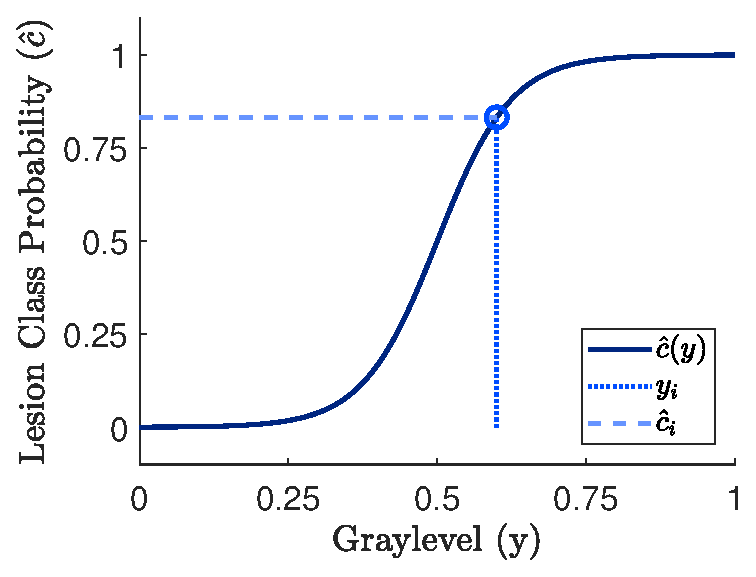
\includegraphics[width=\plotwidth]{lr-basic}
  \caption{The logistic regression model.}%
  \label{fig:lr-basic}
\end{figure}
In the OASIS algorithm~\cite{Sweeney2013,Sweeney2013a}
and the algorithm by \citeauthor{Zhan2017}~\cite{Zhan2017},
this model is used with a number of different graylevel features.
However, this ignores spatial location%
\footnote{The OASIS model also uses Gaussian-blurred images as features,
  which could add some spatial information,
  but this is different from an explicit global context like $x$.}
and therefore makes two assumptions:
first, that graylevels are monotonically related to the lesion class
-- i.e.\ that WMH are either the brightest or darkest class in the image --
and second, that the distribution of graylevels alone is sufficient to discriminate classes.
From the graylevel modelling results in \S~\ref{s:simflair},
it can be shown that typical selections of T1 and T2 imaging parameters
do not create monotonic relationships between graylevel and class label,
contrast between GM and WMH graylevel distributions
is often only around 40\%, even in FLAIR images.
Moreover, these results are derived from ideal conditions;
considering image noise, PVE, imperfect bias field correction, and possible tissue heterogeneity,
the plausibility of class separability by graylevel alone is further diminished.
Again, the potential utility of spatial features is highlighted.
% --------------------------------------------------------------------------------------------------
\subsubsection{Lesion Prediction Algorithm}\label{sss:limits-lpa}
An alternative approach by \citeauthor{Schmidt2017a} aims to solve this issue
by introducing a spatial effect parameter, namely the intercept $\b^0 \rightarrow \b^0(x)$,
which is defined uniquely for each location -- i.e.\ voxel $x$ -- in the imaged volume.
In this method, a Gaussian MRF model is used to estimate the spatial parameter $\b^0(x)$,
while the other $\b$ parameters
-- in fact there is only one: $\b^1$, corresponding to the FLAIR graylevel --
are fixed for the entire image.
A pre-trained version of this method was released as
the \tool{Lesion Prediction Algorithm} (LPA) in the LST toolbox.%
\footnote{\hreftt{http://www.applied-statistics.de/lst.html}}
\par
This particular parametrization has significant implications for model estimation, however,
since $\b^0(x)$ should be estimated uniquely for every spatial location,
but $\b^1$ should consider evidence from the entire image volume.
Efficient fitting of such models was the subject of major works
by~\citeauthor{Schmidt2017}~\cite{Schmidt2017a,Schmidt2017}, but several drawbacks remain.
First, Markov Chain Monte Carlo estimation of the model
appears to create discontinuity artifacts in the spatial effect image $\b^0(x)$
(cf.~Figure~\ref{fig:beta-lpa}, \S~\ref{ss:exp-beta}).
Second, MRF modelling of the parameter images assumes that the missing data
(i.e.\ WMH training examples in the more superficial brain regions)
can be interpolated spatially, but this may not be justified.
Third, this joint estimation procedure is computationally expensive
(versus the methods proposed here),
requiring approximately two hours to estimate $\bb$
to only about 90\% convergence~\cite{Schmidt2017a}.
Finally, it is not clear whether any tied $\b$ are necessary or advantageous in this context.
These deficiencies then motivate investigations into alternative solutions to the above challenges.
\par
In addition to these potential modelling weaknesses, there were also several limitations
to the validation methodology for the LPA algorithm worth noting here.
First, the ``ground truth'' segmentations were generated using an automated algorithm
-- the Lesion Growth Algorithm (LGA)~\cite{Schmidt2012} of the same toolbox --
rather than a human expert.
Second, the graylevel standardization procedure employed does not consider
the variance of image graylevels (only the mean is subtracted);
this strongly assumes that user images will have graylevels spanning a similar range.
Third, all 53 training cases were obtained on the same MRI scanner,
which may limit generalization performance.
Finally, no segmentation performance results
are given in either of the associated publications~\cite{Schmidt2017a,Schmidt2017}.
Therefore, while the open-source release of the LPA algorithm is greatly appreciated,
significant improvements can be made to this algorithm.
%%%%%%%%%%%%%%%%%%%%%%%%%%%%%%%%%%%%%%%%%%%%%%%%%%%%%%%%%%%%%%%%%%%%%%%%%%%%%%%%%%%%%%%%%%%%%%%%%%%%
\section{Proposed Algorithm}\label{s:intro-proposed}
This section presents a brief overview of the proposed WMH segmentation method.
\par
For several reasons, the supervised pipeline approach
was selected as the framework for this algorithm.
First, preliminary work drawing on existing algorithms~\cite{Khademi2014,Schmidt2015}
showed the feasibility of several relatively simple FLAIR-only methods,
which confer robustness and interpretability through simplicity.
Second, the parametric assumptions required by unified probabilistic models
may be challenged by data from multiple sources~\cite{VanLeemput2001}.
Third, only a small number of training cases were available during initial development,
which limited the feasibility of deep learning approaches.
Finally, time constraints favoured the incorporation of existing tools
to address challenges like bias correction and image registration,
which would have been otherwise difficult to develop in a unified model.
\par
The proposed pipeline can be summarized as follows.
Pre-processing steps will aim to
correct any bias field effect, standardize spatial coordinates, and also image graylevels,
since the classification model assumes these features are drawn from a consistent distribution.
The classification model will then employ
the standardized FLAIR intensities and spatial features to give the initial segmentation.
Finally, post-processing steps will generally aim to further improve segmentation performance.
This pipeline is illustrated in Figure~\ref{fig:pipeline}.
Next, the proposed classification model is introduced.
\begin{figure}
  \centering\scalebox{0.65}{\pgfdeclarelayer{background}
\pgfdeclarelayer{foreground}
\pgfsetlayers{background,main,foreground}
\tikzset{%
  arrow/.style = { ->, >=Latex,  very thick, rounded corners, draw = #1!60!white },
  tbox/.style  = { fill = white, draw = #1!60!white, very thick, align = center }
}
\newcommand*{\textbox}[6]{%
  \node[tbox=#5,minimum width=#3cm,minimum height=#4cm]at(#1,#2){#6};
}

\newcommand*{\ix}{0.8}\newcommand*{\ixx}{1.6}
\newcommand*{\iy}{1}  \newcommand*{\iyy}{2}
\newcommand*{\pw}{1.5}
\newcommand*{\fw}{0.3}

% --------------------------------------------------------------------------------------------------
\begin{tikzpicture}
    \useasboundingbox(0.0, 0.0) rectangle (24.0,  2.0);
    \draw[black!30!white,rounded corners,very thick](00.0, 00.0) rectangle (24.0,  2.0);
    \textbox{ 2.0}{ 1.0}{3}{1}{black} {FLAIR MRI}
    \textbox{ 6.0}{ 1.0}{3}{1}{blue}  {Bias Correction\\\& Registration}
    \textbox{10.0}{ 1.0}{3}{1}{violet}{Graylevel\\Standardization}
    \textbox{14.0}{ 1.0}{3}{1}{red}   {Lesion\\Classification}
    \textbox{18.0}{ 1.0}{3}{1}{orange}{Post-Processing}
    \textbox{22.0}{ 1.0}{3}{1}{black} {Label Image}
    \draw[arrow={black}  ]( 3.5, 1.0)--( 4.5, 1.0);
    \draw[arrow={black}  ]( 7.5, 1.0)--( 8.5, 1.0);
    \draw[arrow={black}  ](11.5, 1.0)--(12.5, 1.0);
    \draw[arrow={black}  ](15.5, 1.0)--(16.5, 1.0);
    \draw[arrow={black}  ](19.5, 1.0)--(20.5, 1.0);
%    \draw[arrow={black} ]( 3.5, 1.0)--( 4.5, 1.0);
%    \draw[arrow={blue}  ]( 7.5, 1.0)--( 8.5, 1.0);
%    \draw[arrow={violet}](11.5, 1.0)--(12.5, 1.0);
%    \draw[arrow={red}   ](15.5, 1.0)--(16.5, 1.0);
%    \draw[arrow={orange}](19.5, 1.0)--(20.5, 1.0);
\end{tikzpicture}}
  \caption{Overview of the necessary processing steps.}%
  \label{fig:pipeline}
\end{figure}
% ==================================================================================================
\subsection{Voxel-Wise Logistic Regression}\label{ss:intro-vlr}
The classification model proposed here is similar to the LPA model.
However, several modifications are made
to address the challenges outlined in \S~\ref{sss:limits-lpa}.
Most significantly, spatial variation of \textit{all} logistic parameters is now permitted,
yielding a separate logistic regression model for each voxel
-- i.e. ``Voxel-wise Logistic Regression'' (VLR).
Mathematically, this is
\begin{equation}
  P\big(c(x)=1\mid\by(x);\bb(x)\big) = \frac{1}{1+e^{-\eta(x)}},\qquad\eta = {\bb(x)}^T\bm{Y}(x).%
  \label{eq:eq:vlrmodel-intro}
\end{equation}
Training the VLR model then yields a complete and unique vector $\bb$ for each voxel $x$,
or equivalently, one complete image for each parameter.
Only one additional $\b$ is used here, again corresponding to the FLAIR graylevel.
This formulation allows completely independent estimation of the logistic model for each voxel $x$,
facilitating improved estimates.
In turn, this permits essentially complete convergence in significantly less time,
and does not require sampling approximations or smoothness assumptions
(though methods of enforcing smoothness post hoc will be explored).
\par
Overall, the VLR model solves the problem of unreliable separability by graylevel alone,
and presents a method for differential treatment of spatial and graylevel features
(versus K-NN, etc.).
That is, the characteristics of the logistic regression model
are maintained with respect to graylevel features,
but spatial features can have more complex relationships (non-monotonic) with the output.
The estimated VLR parameters are also highly interpretable,
allowing prior knowledge to guide improved regularizations versus those used in the LPA algorithm.
Different pre- and post-processing methods versus the LPA algorithm are also developed.
%%%%%%%%%%%%%%%%%%%%%%%%%%%%%%%%%%%%%%%%%%%%%%%%%%%%%%%%%%%%%%%%%%%%%%%%%%%%%%%%%%%%%%%%%%%%%%%%%%%%
\section{Contributions}
This thesis aims to produce a WMH segmentation algorithm
which can be used on FLAIR MRI from any source,
and to characterize the expected performance on unseen data.
The major contributions are as follows:
\begin{enumerate}
  \item A review and critique of the previously proposed WMH segmentation algorithms,
  especially with respect to expected performance on unseen data;
  \item Voxel-Wise Logistic Regression (VLR): a new FLAIR-only WMH segmentation algorithm;
  \item Leave-One-Source-Out Cross Validation (LOSO-CV): a validation framework
  which accurately characterizes the generalization performance of medical image analysis methods;
  \item Extensive validation of the proposed method and its components.
\end{enumerate}
The remainder of this thesis is organized as follows:
Chapter~\ref{ch-pre} explores the pre-processing steps
required to satisfy the assumptions of the VLR model.
Chapter~\ref{ch-vlr} develops the voxel-wise logistic regression model,
including expected challenges and regularization solutions with this approach;
Chapter~\ref{ch-exp} explores optimization of model components through experimentation,
and then presents segmentation performance results under various cross validation schemes;
Chapter~\ref{ch-conc} draws conclusions about the work,
and highlights avenues for future investigation.
% --------------------------------------------------------------------------------------------------
% ==================================================================================================
%%%%%%%%%%%%%%%%%%%%%%%%%%%%%%%%%%%%%%%%%%%%%%%%%%%%%%%%%%%%%%%%%%%%%%%%%%%%%%%%%%%%%%%%%%%%%%%%%%%%
